\documentclass{mwrep}

% Polskie znaki
\usepackage{polski}
\usepackage[polish]{babel}
\usepackage[utf8]{inputenc}
\usepackage[T1]{fontenc}
\usepackage[utf8]{luainputenc}
\usepackage{lmodern}
\usepackage{indentfirst}

% Strona tytułowa
\usepackage{pgfplots}
\usepackage{siunitx}
\usepackage{paracol}
\usepackage{gensymb}

% Pływające obrazki
\usepackage{float}
\usepackage{svg}
\usepackage{graphicx}

% table of contents refs
\usepackage{hyperref}
\usepackage{cleveref}
\usepackage{booktabs}
\usepackage{listings}
\usepackage{placeins}
\usepackage{xcolor}

\usetikzlibrary{pgfplots.groupplots}
\sisetup{detect-weight,exponent-product=\cdot,output-decimal-marker={,},per-mode=symbol,binary-units=true,range-phrase={-},range-units=single}
\definecolor{szary}{rgb}{0.95,0.95,0.95}
%konfiguracje pakietu listings
\lstset{
	backgroundcolor=\color{szary},
	frame=single,
	breaklines=true,
}
\lstdefinestyle{customlatex}{
	basicstyle=\footnotesize\ttfamily,
	%basicstyle=\small\ttfamily,
}

\lstdefinestyle{customjs}{
  keywords={typeof, new, true, false, catch, function, return, null, catch, switch, var, if, in, while, do, else, case, break},
  keywordstyle=\color{blue}\bfseries,
  ndkeywords={class, export, boolean, throw, implements, import, this},
  ndkeywordstyle=\color{darkgray}\bfseries,
  identifierstyle=\color{black},
  sensitive=false,
  comment=[l]{//},
  morecomment=[s]{/*}{*/},
  commentstyle=\color{purple}\ttfamily,
  stringstyle=\color{red}\ttfamily,
  morestring=[b]',
  morestring=[b]",
  basicstyle=\footnotesize\ttfamily,
  extendedchars=true,
  showstringspaces=false,
}

\lstdefinestyle{customc}{
	breaklines=true,
	frame=tb,
	language=C,
	xleftmargin=0pt,
	showstringspaces=false,
	basicstyle=\small\ttfamily,
	keywordstyle=\bfseries\color{green!40!black},
	commentstyle=\itshape\color{purple!40!black},
	identifierstyle=\color{blue},
	stringstyle=\color{orange},
}
\lstdefinestyle{custommatlab}{
	%basicstyle=\fontsize{11}{13}\selectfont\ttfamily,
	captionpos=t,
	breaklines=true,
	frame=tb,
	xleftmargin=0pt,
	language=matlab,
	showstringspaces=false,
	%basicstyle=\footnotesize\ttfamily,
	basicstyle=\scriptsize\ttfamily,
	keywordstyle=\bfseries\color{green!40!black},
	commentstyle=\itshape\color{purple!40!black},
	identifierstyle=\color{blue},
	stringstyle=\color{orange},
}

%wymiar tekstu
\def\figurename{Rys.}
\def\tablename{Tab.}

%konfiguracja liczby p�ywaj�cych element�w
\setcounter{topnumber}{0}%2
\setcounter{bottomnumber}{3}%1
\setcounter{totalnumber}{5}%3
\renewcommand{\textfraction}{0.01}%0.2
\renewcommand{\topfraction}{0.95}%0.7
\renewcommand{\bottomfraction}{0.95}%0.3
\renewcommand{\floatpagefraction}{0.35}%0.5

\SendSettingsToPgf
\title{\bf Prezentacja i omówienie architektury modułu ESP8266 \vskip 0.1cm}
\author{Jakub Sikora}
\date{\today}
\pgfplotsset{compat=1.15}	
\begin{document}
\frenchspacing
\pagestyle{uheadings}

\makeatletter
\renewcommand{\maketitle}{\begin{titlepage}
		\begin{center}{
				\LARGE {\bf Politechnika Warszawska}}\\
            \vspace{0.4cm}
            \leftskip-0.9cm
            {\LARGE {\bf \mbox{Wydział Elektroniki i Technik Informacyjnych}}}\\
            \vspace{0.2cm}
            {\LARGE {\bf \mbox{Instytut Automatyki i Informatyki Stosowanej}}}\\
            
            \vspace{5cm}
            \leftskip-2cm
			{\bf \Huge \mbox{Zaawansowane architektury procesorów} \vskip 0.1cm}
		\end{center}
		\vspace{0.1cm}

		\begin{center}
			{\bf \LARGE \@title}
		\end{center}

		\vspace{9cm}
		\begin{paracol}{2}
			\addtocontents{toc}{\protect\setcounter{tocdepth}{1}}
			\subsection*{Autor:}
			\bf{ \Large{ \noindent\@author \par}}
			\addtocontents{toc}{\protect\setcounter{tocdepth}{2}}

			\switchcolumn \addtocontents{toc}{\protect\setcounter{tocdepth}{1}}
			\subsection*{Prowadzący:}
			\bf{\Large{\noindent \mbox{mgr inż. Grzegorz Mazur}}}
			\addtocontents{toc}{\protect\setcounter{tocdepth}{2}}

		\end{paracol}
		\vspace*{\stretch{6}}
		\begin{center}
			\bf{\large{Warszawa, \@date\vskip 0.1cm}}
		\end{center}
	\end{titlepage}
}
\makeatother
\maketitle
\tableofcontents

\chapter{Omówienie architektury modułu ESP8266}
\label{omowienie_arch}

\section{Opis modułu}
\label{opis_modulu}

ESP8266 jest tanim modułem umożliwiającym komunikację przez Wi-Fi.
Oferuje on pełną obsługę protokołu TCP/IP a także funkcjonalność prostego
32 bitowego mikrokontrolera. Jest naturalnym następcą modułu ESP32. Niska cena 
i mały rozmiar sprawiły że stał się on bardzo popularny wśród konstruktorów 
urządzeń internetu rzeczy.\\

\begin{figure}[H]
	\centering
    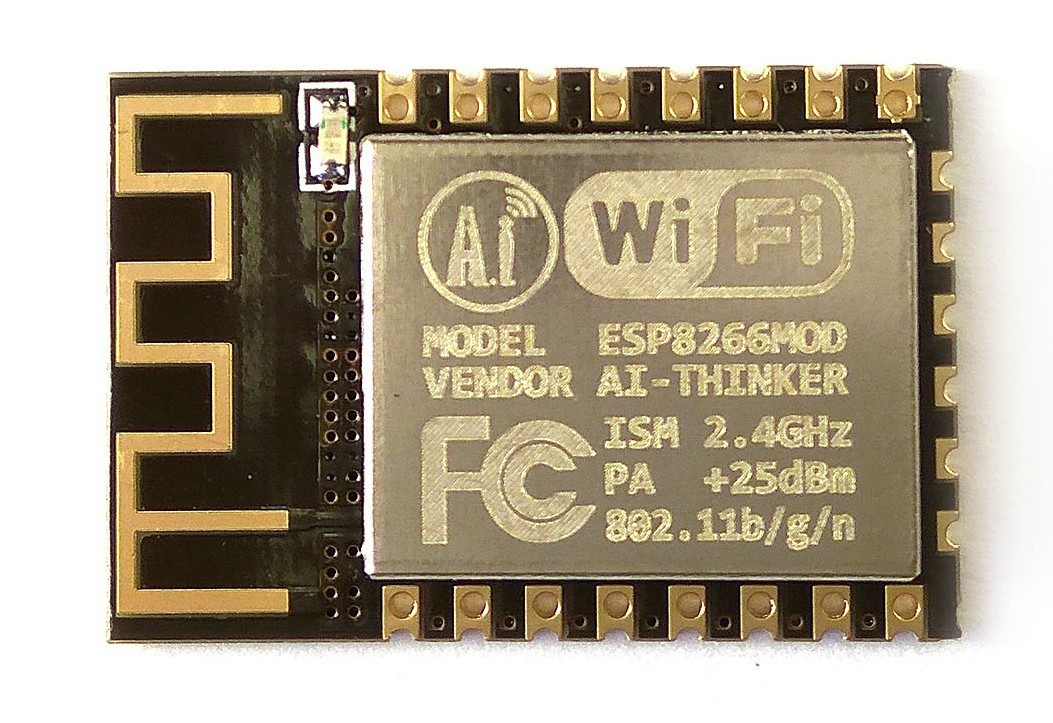
\includegraphics[width=8cm]{./images/esp8266.jpg}
    \caption{Moduł ESP8266 w podstawowej wersji ESP8266-12F firmy AI Thinker}
	\label{esp8266}
\end{figure}

\subsection{Mikroprocesor}
\label{mikroprocesor}

Na pokładzie modułu ESP8266 znajduje się 32 bitowy mikroprocesor z architektury RISC, 
bazowany na standardzie Xtensa Diamond Standard 106Micro firmy Tensilica.
Jest on domyślnie taktowany zegarem $\num{80}$ MHz, którego częstotliwość można 
zwiększyć do $\num{160}$ MHz. Mikroprocesor został tak skonstruowany aby pobierać 
możliwie jak najmniej energii, przez co dostępne są trzy tryby pracy:
\begin{itemize}
    \item \textit{active mode} 
    \item \textit{sleep mode}
    \item \textit{deep sleep mode}
\end{itemize}
W trybie \textit{deep sleep mode} moduł pobiera około $\num{60}$ \si{\micro A}, co pozwala
na bardzo długą pracę urządzenia zasilanego z baterii.


\subsection{Organizacja pamięci}
\label{pamiec}
Moduł ESP8266 został wyposażony w wbudowaną pamięc SRAM oraz ROM. Rozmiar dostępnej
pamięci RAM dla programu użytkownika w przypadku podłączenia do sieci Wi-Fi w trybie
\textit{station mode} wynosi około $\num{80}$ KiB. Docelowo 
pamięc RAM dostępna dla użytkownika rozpoczyna się od adresu \texttt{3FFE8000h}.
Ten obszar pamięci służy do przechowywania aktualnie obrabianych danych, jest to typowa 
pamięć operacyjna modułu.
Wewnętrzna pamięć ROM nie jest programowalna a jej rozmiar wynosi $\num{64}$ KiB.
Pamięć ROM mapowana jest w taki sposób że rozpoczyna się od adresu \texttt{40000000h}.
W pamięci ROM znajduje się bootloader, który obsługuje pobieranie nowego programu poprzez
UART oraz zajmuje się jego wykonywaniem z pamięci Flash. W pamięci ROM znajujde się także 
implementacja podstawowych funkcji systemowych typu \texttt{alloc} czy \texttt{memcpy}.

\begin{figure}[H]
	\leftskip3cm
    \includegraphics[width=8cm]{./images/memorymap.pdf}
    \caption{Uproszczona mapa pamięci modułu ESP8266}
	\label{memmap}
\end{figure}

Oprócz wbudowanej pamięci, na pokładzie modułu znajduje się również zewnętrzna programowalna
pamięć Flash do przechowywania programów użytkownika. Według dokumentacji, istnieje
możliwość podłączenia pamięci o maksymalnym rozmiarze $\num{16}$ MiB. Zakłada się 
że minimalny rozmiar pamięci Flash powinien wynosić $\num{512}$ KiB w przypadku wyłaczonej
funkcjonalności OTA (Over The Air Update) i $\num{1}$ MiB przy włączonym OTA. Komunikacja
z pamięcią Flash zachodzi przy pomocy interfejsu SPI.\\

Program wykonywany może zostać również załadowany bezpośrednio do pamięci RAM z pominięciem 
pamięci Flash. Pozwala to na znaczne przyspieszenie działania programu, jednak należy pamiętać 
że w przypadku utraty zasilania, zawartość pamięci RAM zostanie stracona.

\subsection{Wi-Fi}
\label{wifi}
Głównym zastosowaniem modułu ESP8266 jest możliwość komunikowania się urządzenia wbudowanego
z siecią Wi-Fi. Urządzenie oparte na ESP8266 może pełnić trzy role w sieci:\\
\begin{itemize}
    \item \textit{Wireless Access Point (AP)}
    \item \textit{Station}
    \item \textit{AP + Station}\\
\end{itemize}

\textit{Wireless Access Point}, w skrócie AP, to urządzenie które pełni rolę 
hubu komunikacyjnego.  To z AP łączą się urządzenia nazywane stacjami (z ang. \textit{Station}).
AP są najczęściej połączone z internetem, co umożliwia stacjom
bezprzewodowe połaczenie z siecią. ESP8266 może pełnić obie role, wymiennie oraz równocześnie.\\

\begin{figure}[H]
	\centering
    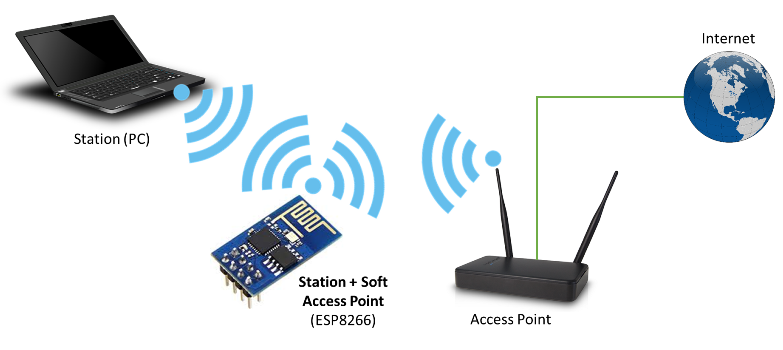
\includegraphics[width=12cm]{./images/WiFi-stationap-mode.png}
    \caption{Praca modułu ESP8266 jako \textit{Access Point} oraz jako \textit{Station}}
    \label{ap+station}
\end{figure}


Komunikacja sieciowa jest obsługiwana przez wewnętrzny kod. Stawia to pewne ograniczenia 
na program użytkownika, wynikające z faktu że w trakcie wykonywania kodu aplikacji 
użytkownika, nie jest wykonywany kod obsługujący komunikację. Brak wątków powoduje że 
kod użytkownika zawsze przerywa obsługę zdarzeń sieciowych. Aby umożliwić poprawne działanie
modułu, należy tak zaprojektować kod użytkownika aby pojedyncze wejście do kodu użytkownika
trwało krócej niż $\num{10}$ ms.\\


Moduł ESP8266 docelowo przechowuje informację o sieci z którą ma się połączyć w pamięci Flash.
Umożliwia to połączenie się z siecią po restarcie urządzenia bez żadnych dodatkowych informacji 
z zewnątrz. Znacznie upraszcza to uruchamianie urządzenia, jednak powoduje że zmiana sieci 
lub tylko hasła do niej wymaga przeprogramowania pamięci. Istnieje jednak możliwość 
nadpisania funkcji automatycznie łączących się z AP \verb+wifi_station_set_auto_connect()+ oraz 
\verb+wifi_station_get_auto_connect()+, tak aby po restarcie pobierały one dane z interfejsu szeregowego.\\

W przypadku pracy w trybie \textit{Station}, urządzenie skanuje dostępne sieci
bezprzewodowe z którymi może się połączyć. Do skanowania została przygotowana 
funkcja \verb+wifi_station_scan()+, która jako argument przyjmuję \textit{callback}
do której jako argument zostanie przekazana lista struktur BSS. Struktura BSS
przechowuje informację o SSID sieci, BSSID powiązanego z danym AP, kanale, mocy
sygnału i wielu innych. Na samym końcu struktury znajduje się wskaźnik na następny 
element listy.\\

Obsługa zdarzeń sieciowych również opiera się na \textit{callback'ach}. Za pomocą 
funkcji \verb+wifi_set_event_handler_cb()+, możemy ustawić która funkcja ma 
obsługiwać zdarzenia sieciowe. Poniżej przedstawiono postać przykładowej funkcji.\\

\begin{lstlisting}[style=customc,
    frame=single,
    caption={Przykładowa postać funkcji obsługującej zdarzenia sieciowe},
    captionpos=b,
    label={event_handler_cb}]
void eventHandler(System_Event_t *event) {
    switch(event->event) {
      case EVENT_STAMODE_CONNECTED:
        os_printf("Event: EVENT_STAMODE_CONNECTED\n");
        break;
      case EVENT_STAMODE_DISCONNECTED:
        os_printf("Event: EVENT_STAMODE_DISCONNECTED\n");
        break;
      default:
        os_printf("Unexpected event: %d\n", event->event);
        break;
    }
}
\end{lstlisting}

\subsection{Interfejsy zewnętrzne}
\label{interfejsy}

\subsubsection{GPIO}
\label{gpio}
Moduł ESP8266 oferuje do 17 typowych pinów wejścia-wyjścia ogólnego przeznaczenia. Piny
te są multipleksowane z innymi funkcjami takimi jak I2C czy PWM, opisanymi w dalszej 
części tego dokumentu. Wszystkie piny mogą zostać skonfigurowane z wewnętrznym 
podciągnięciem do zasilania (\textit{pull-up}), w konfiguracji \textit{push-pull} lub 
\textit{open-drain}. Można skonfigurować piny w taki sposób aby zmiana zbocza zgłaszała
przerwanie do procesora.


\subsubsection{SDIO}
\label{sdio}
Moduł oferuje jeden interfejs \textit{Secure Digital Input Output}, który wykorzystywany
jest do komunikacji z kartami SD a także z innymi urządzeniami obsługującymi ten standard.


\subsubsection{SPI}
\label{spi}
W ESP8266 znalazło się miejsce na sprzętowy interfejs SPI. Możliwe jest połączenie się z jednym
urządzeniem jako master lub jako slave.


\subsubsection{I2S}
\label{i2s}
ESP8266 obsługuje interfejs I2S (\textit{Inter-IC Sound}). W obecnej wersji dostępny
jest jest interfejs wejściowy i jeden interfejs wyjściowy.

\subsubsection{PWM}
\label{pwm}
Na pokładzie modułu znajdują się cztery wyjścia PWM, których funkcjonalność może
być rozszerzana poprzez użytkownika.

\subsubsection{ADC}
Moduł ESP8266 został wyposażony w typowy konwerter analogowo-cyfrowy typu SAR, opierający
się na sukcesywnej aproksymacji sygnału. Konwerter ma 10 bitową dokładność, co oznacza
że może mierzyć sygnały z dokładnością do $\num{3.2}$ \si{mV}. Na płytce znajduje się
tylko jedno wyprowadzenie konwertera, multipleksowane z pinem \verb+GPIO6+.

\subsubsection{UART}
Moduł ESP8266 został zaopatrzony w dwa interfejsy sprzętowe UART. Pierwszy z nich
obsługuje obustronną komunikację, natomiast drugi posiada tylko sygnał Tx, co naturalnie
sprowadza go do funkcji swoistego loggera do wypisywania stanu systemu. Prędkość transmisji
może zostać zwiększona aż do $\num{4.5}$ Mbps. 

W dokumentacji bootloadera znajduje się informacja o logach wypisywanych 
na interfejsie \verb+UART0+, podczas uruchamiania systemu. 
Prędkość transmisji zależy wtedy od częstotliwości
wewnętrznego oscylatora. Jeśli ustawiona jest na bazowe $\num{40}$ \si{MHz} to 
prędkość transmisji wynosi wtedy $\num{115200}$ bps. Należy zwrócić na to uwagę
przy zmniejszaniu częstotliwości oscylatora, w celu zmniejszenia zużycia energii.

\subsubsection{I2C}
Dodatkowo, producent programowo zaimplementował obsługę interfejsu I2C. 
Urządzenie może pełnić rolę Master lub Slave, z takim zastrzeżeniem że zegar
taktujący komunikację może mieć częstotliwość maksymalną $\num{100}$ \si{kHz}.\\


\subsection{Watchdog}
\label{watchdog}

Moduł ESP8266 został wyposażony w systemowego watchdoga sprzętowego oraz
jednego watchdoga realizowanego programowo. Zadaniem watchdoga jest reset urządzenia 
w przypadku sytuacji awaryjnej lub błędu. W pierwszej kolejności reaguje watchdog
programowy, który w przypadku błędu resetuje urządzenie i na porcie szeregowym 
wyrzuca informację o błędzie. W przypadku gdy watchdog programowy nie zareaguje, 
do działania wkracza watchdog sprzętowy. Reset przez watchdog sprzętowy nie powoduje
wypisania informacji o błędzie.\\

Watchdogi w ESP8266 pilnują aby kod użytkownika nie wykonywał się zbyt długo, ponieważ
w momencie wykonywania kodu użytkownika, nie wykonuje się kod obsługujący komunikację 
przez Wi-Fi.
\chapter{Organizacja oprogramowania}
\label{organizacja_opr} 


\section{ESP8266 RTOS SDK}
\label{sdk}
W ramach projektu, za stroną producenta, zdecydowałem się na skorzystanie z 
szkieletu aplikacyjnego \verb+ESP8266_RTOS_SDK+, wykorzystującego FreeRTOS.
Takie podejście pozwala na pisanie prostych aplikacji wielozadaniowych. Dodatkowo, 
szkielet udostępnia rozbudowane API, które znacznie upraszcza korzystania z peryferiali oraz sieci Wi-Fi. 

\subsection{Instalacja środowiska}
\label{instalacja}
Dużą zaletą środowiska \verb+ESP8266_RTOS_SDK+ przygotowanego przez firmę \textit{Espressif}
jest prostota instalcji i korzystania z niego. Środowisko można pobrać ze strony producenta
lub z publicznego repozytorium znajdującego się w serwisie \verb+github.com+. Po instalacji
i ustawieniu koniecznych zmiennych środowiskowych, można przystąpić do wgrania programu.

\subsection{Tworzenie programu}
\label{tworzenie programu}
W celu stworzenia własnego aplikacji na moduł \verb+ESP8266+ należy skopiować folder 
\verb+project_template+ do wybranego folderu i w pliku \verb+user_main.c+ zapisać swój kod
źródłowy. Struktura przykładowego programu została przedstawiona w \ref{example_C}.

\subsection{Kompilacja i wgranie programu}
\label{kompilacja}
Środowisko znacząco upraszcza pracę nad aplikacjami, ponieważ dostarcza plik \verb+Makefile+
który samemu zajmuje się kompilacją i wgrywaniem programu. Z poziomu programisty, należy jedynie
wywołać polecenie \texttt{make flash}, które kolejno wywoła kompilator \verb+xtensa-lx106-elf-gcc+
a następnie narzędzie do wgrywania \verb+esptool.py+ napisane w języku Python.

W przypadku zwykłych modułów, konieczne jest ręczne ustawienie określonych pinów GPIO w taki sposób
aby przy resecie urządzenia przeszło ono w tryb UART, pozwalający programować pamięc Flash.
Po wgraniu programu, należy zresetować urządzenie, tak aby uruchomić bootloader w trybie FLASH, 
pozwalający na normalną pracę urzadzenia. Oprócz tego, istnieje jeszcze tryb SD, umożliwiający 
uruchomienie systemu z karty SD. Sposób ustawienia pinów został przedstawiony w tabeli 
\ref{tabela_trybow}

\begin{table}[H]
    \centering
    \begin{tabular}{lccc}
    \hline
          & \multicolumn{1}{l}{GPIO0} & \multicolumn{1}{l}{GPIO2} & \multicolumn{1}{l}{GPIO15} \\ \hline
    UART  & 0                         & 1                         & 0                          \\
    FLASH & 1                         & 1                         & 0                          \\
    SD    & x                         & x                         & 1                         
    \end{tabular}
    \caption{Porównanie pinów badanych przez bootloader podczas uruchamiania systemu}
    \label{tabela_trybow}
\end{table}
\FloatBarrier
\newpage
W przypadku modułu ESP8266-EVB użyczonego z zasobów Instytutu Informatyki w ramach tego projektu,
producent umieścił na płytce przycisk pozwalający na ustawienie omawianych pinów
w odpowiedni sposób tak aby przy włączeniu urządzenia przy wciśniętym przycisku, wchodził
on w tryb UART.

\begin{figure}[H]
	\centering
    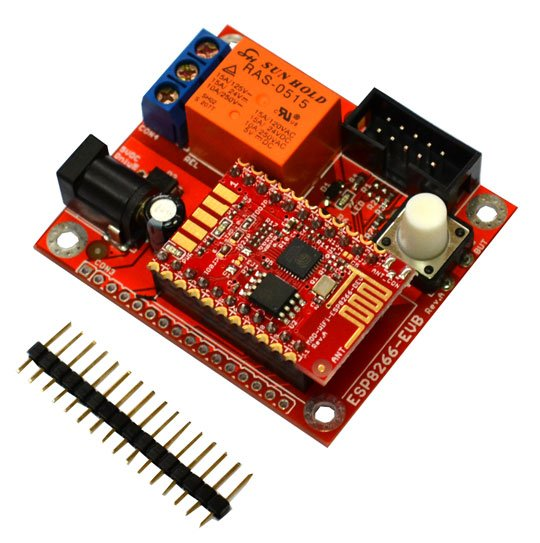
\includegraphics[width=8cm]{./images/ESP8266-EVB.jpg}
    \caption{Płytka ESP8266-EVB firmy OLIMEX}
	\label{esp8266-evb}
\end{figure}
\FloatBarrier

W przypadku finalnie wykorzystanego przeze mnie modułu NodeMCU w wersji 3 z modułem
ESP8266, nie było potrzeby ręcznego przestawiania trybu pracy. Wszystkim tym zajmowało
się program do wgrywania kodu. Znacznie ułatwiało i przyspieszało to pracę nad projektem.
Płytka ta jest zasilana z kabla USB, który podpięty do komputera służył również do komunikacji
przez port szeregowy.

\begin{figure}[H]
	\centering
    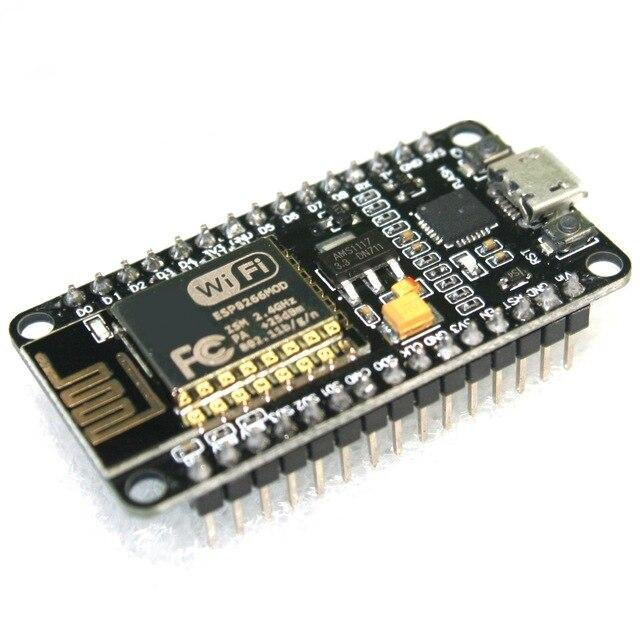
\includegraphics[width=8cm]{./images/nodemcu.jpg}
    \caption{Wykorzystana płytka ewaluacyjna NodeMCU v3}
	\label{esp8266-nodemcu}
\end{figure}
\FloatBarrier

\subsection{Narzędzie \texttt{esptool.py}}
\label{esptool}
Narzędzie \texttt{esptool.py} umożliwia prgoramowanie modułu ESP8266. Zostało one 
napisane w języku Python w wersji 2. Aby zaprogramować płytkę należy wywołać 
program z odpowiednimi argumentami. Przykładowa komenda wygląda w następujący sposób:

\begin{lstlisting}[style=customc,
    frame=single,
    caption={Przykładowa komenda programująca moduł ESP8266},
    captionpos=b,
    label={esptool_basic}]
esptool.py --port COM4 write_flash 0x1000 my_app-0x01000.bin
\end{lstlisting}

Po komendzie \texttt{write\_{}flash} należy zapisać adres początkowy programu w 
pamięci Flash. Program umożliwia również konwersję plików \texttt{.elf} do postaci 
binarnej \texttt{.bin}. 

\texttt{esptool.py} pozwala również załadować program do pamięci RAM, tak jak to było
wspomniane w \ref{pamiec}. Aby w ten sposób wgrać program, należy skorzystać z polecenia 
\texttt{load\_{}ram}.

\section{Budowa przykładowego programu w języku C}
\label{example_C}


\chapter{Projekt czujnika opartego o moduł ESP8266 napisany w języku C}
\label{projekt}

\chapter{Przegląd pozostałych możliwości wykorzystania modułu}
\label{inne}

W tym rozdziale przedstawione zostały inne możliwości programowania 
modułu ESP8266. Język C ma to do siebie że jest językiem pozostającym 
blisko sprzętu, co może uprzykrzać życie hobbystom lub początkującym
konstruktorom urządzeń internetu rzeczy. Aby ułatwić programowanie, 
powstał szereg różnych wysokopoziomowych rozwiązań znacząco upraszczające 
korzystanie z modułu.

\section{Wykorzystanie języka skryptowego Lua}
\label{lua}
Po wgraniu specjalnego programu NodeMCU do pamięci Flash modułu,
możemy programować w języku skryptowym Lua. Programowanie odbywa się wtedy
z poziomu Arduino IDE.\\

Skrypty mogą być wgrywane jako pliki \verb+.lua+ lub pisane i wykonywane na bieżąco
tak jak na przykład w przypadku interpretera języka Python. Język Lua cechuje się 
olbrzymią prostotą i szybkością programowania. Przykładowo połączenie się z wifi 
wymaga dwóch linijek kodu:\\

\begin{lstlisting}[style=customjs,
    frame=single,
    caption={Kod łączący się z siecią Wi-Fi napisany w języku Lua},
    captionpos=b,
    label={lua_example}]
wifi.setmode(wifi.STATION)
wifi.sta.config("SSID","HASLO")
\end{lstlisting}

Prostota języka zachęca do korzystania z niego przy pisaniu aplikacji internetu 
rzeczy. Niestety jako język wysokopoziomowy, jest mocno oddzielony od sprzętu i nie 
pozwala na zrozumienie architektury modułu. Po resecie urządzenia, oprogramowanie szuka
zapisanego pliku \texttt{init.lua} z programem użytkownika.

\section{Wykorzystanie MicroPythona}
\label{micropython}
Korzystanie z MicroPythona jest bardzo podobne do korzystania z NodeMCU. W pierwszej
kolejności należy wgrać interpreter na moduł ESP8266. Po resecie, oprogramowanie szuka
pliku \texttt{main.py} z programem użytkownika.
Język programowania wykorzystywany w MicroPythonie różni się nieznacznie od zwykłego
Pythona w wersji 3. Różnice są jednak niewielkie, dlatego jeżeli ktoś zna Pythona to
bardzo łatwo jest mu zaprogramować urządzenie. Poniżej znajduje się kod 
do połączenia modułu z siecią Wi-Fi.

\begin{lstlisting}[style=custompython, caption={Przykładowy kod do 
    połączenia się z siecią Wi-Fi w języku MicroPython},
    captionpos=b]
import network
wlan = network.WLAN(network.STA_IF)
wlan.active(True)
if not wlan.isconnected():
    print('connecting to network...')
    wlan.connect('essid', 'password')
    while not wlan.isconnected():
        pass
\end{lstlisting}


 
\section{AT Commands}
\label{AT}
Aby wykorzystać moduł ESP8266 do połaczenia się z siecią Wi-Fi, nie jest wymagana
umiejętność programowania urządzenia. Większość urządzeń z pudełka przychodzi z wgranym
programem ESP8266 AT Firmware, który pozwala na łączenie sie modułu z siecią Wi-Firmware
za pomocą specjalnych komend AT. Zasada korzystania z modułu jest prosta. Urządzenie 
nadrzędne wysyła poprzez port szeregowy komendę a następnie przez port szeregowy odbiera dane.
Moduł ESP8266 pełni rolę pośrednika w komunikacji. Na poniższym listingu znajduje się 
kod na Arduino, który uruchamia serwer HTTP za pośrednictwem modułu.\\

\begin{lstlisting}[style=customc,
    frame=single,
    caption={Kod uruchamiający serwer HTTP na płytce Arduino z wykorzystaniem modułu ESP8266},
    captionpos=b,
    label={projekt_adc_task}]
sendData("AT+RST\r\n",500,DEBUG); 
sendData("AT+CWMODE=2\r\n",500,DEBUG); 
sendData("AT+CIFSR\r\n",500,DEBUG);
sendData("AT+CIPMUX=1\r\n",500,DEBUG); 
sendData("AT+CIPSERVER=1,80\r\n",500,DEBUG); 
\end{lstlisting}

W pierwszej kolejności urządzenie nadrzędne resetuje moduł i przestawia go w tryb 
\textit{Access Point}. Następnie konfiguruje moduł tak aby uzyskał adres IP oraz 
umożliwił połączenie wielu stacjom. Ostatnia komenda uruchamia serwer.



\begin{thebibliography}{1}
    \bibitem{datasheet}
    Espressif Systems 
    \textit{ESP8266 Datasheet}.\\
    \texttt{https://bbs.espressif.com}, 2015.\\

    \bibitem{reference}
    Espressif Systems
    \textit{ESP8266 Technical Reference}.\\
    \texttt{https://bbs.espressif.com}, 2017.\\

    \bibitem{kolban}
    Neil Kolban.
    \textit{Kolban's Book on the ESP32 \& ESP8266}. \\
    \texttt{https://www.neilkolban.com/tech/}, Texas, USA, 2016.\\

    \bibitem{olimex}
    OLIMEX \textsuperscript{\textcopyright}.
    \textit{How to use ESP8266 with Arduino IDE}.\\
    \texttt{https://www.olimex.com/}, 2017.\\

    \bibitem{at_instruction_set}
    Espressif Systems.
    \textit{ESP8266. AT Instruction Set}.\\
    \texttt{https://www.espressif.com}, 2019.\\

    \bibitem{espressif_guide}
    Espressif Systems.
    \textit{ESP8266 SDK. Getting Started Guide}.\\
    \texttt{https://www.espressif.com}, 2019.\\

\end{thebibliography}




\end{document}